\documentclass[a4paper,12pt]{article}

\usepackage[utf8]{inputenc}
\usepackage{amsmath}
\usepackage{amsfonts}
\usepackage{amssymb}
\usepackage{graphicx}
\usepackage{wrapfig}
\graphicspath{ {./images/} }
\usepackage[hidelinks]{hyperref}
\usepackage[style=numeric]{biblatex}
\addbibresource{refs.bib}

\title{Fuzzer Research}
\author{Jack Foley}
\date{\today}

\begin{document}

\pagenumbering{gobble}
\maketitle

\newpage
\pagenumbering{roman}
\tableofcontents
\listoffigures

\newpage
\pagenumbering{arabic}

\section{Introduction}
This document will outline the research done to start the work on the 4th Software Development Final Year Project (FYP). This project was created by Dr. Chris Meudec and is based on the idea of creating a fuzzer for the C programming language.

\section{Fuzzing}


Fuzzing is a method of testing software by using broken, random or unusual data as an input 
into the software which is being tested. The idea of fuzzing is that it will find bugs and 
other issues, such as memory spikes and leaks (temporary denial-of-service), buffer overruns 
(remote code execution), unhandled exceptions, read access violations (AVs), and thread 
hangs (permanent denial-of-service). These are issues that traditional software testing 
methods, such as unit testing, will not find as easily. There are some different types of 
fuzzing, such as white-box, grey-box and black-box fuzzing \cite{neystadt2009}.

\begin{wrapfigure}{r}{0.5\textwidth} %this figure will be at the right
    \centering
    \caption{American Fuzzy Lop screenshot. Version used: 1.86b \cite{enwiki:1249540069}}
    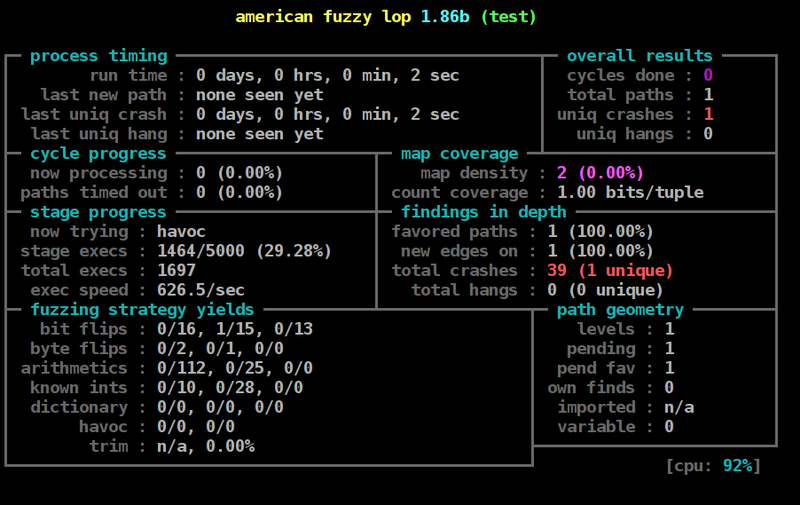
\includegraphics[width=0.5\textwidth]{afl.png}
\end{wrapfigure}

During typical use of a fuzzer, the fuzzer will use structured data as its input. The 
structure that the fuzzer will use is normally already defined via "a file format or 
protocol" \cite{enwiki:1249540069} which in turn can be used to determine a correct input
from an incorrect input. The fuzzer will create cases that are considered 
'correct enough' so that the software will not reject it, but also 'incorrect enough' so 
that "corner cases" \cite{enwiki:1249540069} can be found.


\subsection{White-box Fuzzing}
White-box fuzzing, also known as smart fuzzing, is a technique that is used where the fuzzer is fully aware of the code structure and input variables. White-box fuzzing can lead to discovering bugs more quickly compared to grey-box and black-box fuzzing, but it can also be more computationally expensive as it needs to do an analysis of the codebase before running. 

A case study done during development of ISA Server 2006 showed that one defect was found per 17 KLOC (thousand lines of code), a similar black-box fuzzer only found 30\% of the defects that the white-box fuzzer found \cite{neystadt2009}.

\subsection{Black-box Fuzzing}
Black-box fuzzing is a technique used to test software, analyzing the software by sending random data to the software to discover an application's bugs and vulnerabilities. The black-box fuzzer does not have any information about the inner-workings of the software, it only knows the input and output of the software.


It is a sought-after testing technique as it will work it applications regardless of the programming language or the platform that the software is running on \cite{ALSAEDI202210068}.

\subsection{Grey-box Fuzzing}
Grey-box fuzzing is a well-known and commonly used fuzzing technique that is used for testing software and finding vulnerabilities. Differing from white-box fuzzing, which can suffer from high computational needs since source code analysis is required, grey-box fuzzing is a very good middle-ground between white-box and black-box fuzzing.\cite{8839290} 

Grey-box fuzzing can also receive coverage feedback from the software, which can then be used to more efficiently traverse the software's codebase to find bugs and vulnerabilities  \cite{Blackwell2024-ao}.

\newpage

\printbibliography

\end{document}